% =====================================================================
%  Proposta de Projeto — Oficina de Integração — UTFPR Pato Branco
%  Hologram Orbiter: display volumétrico por persistência de visão
%  Compilar com: tectonic proposta.tex
% =====================================================================
\documentclass[10pt,a4paper,twocolumn]{article}

\usepackage[T1]{fontenc}
\usepackage[utf8]{inputenc}
\usepackage[brazil]{babel}
\usepackage{lmodern}
\usepackage[a4paper,top=2.2cm,bottom=2.2cm,left=2.0cm,right=2.0cm,
            columnsep=0.7cm]{geometry}
\usepackage{amsmath,amssymb}
\usepackage{graphicx}
\usepackage{booktabs}
\usepackage{tikz}
\usepackage{xcolor}
\usepackage[font=small,labelfont=bf,skip=4pt]{caption}
\usepackage{enumitem}
\usepackage{titlesec}
\usepackage{abstract}
\usepackage[hidelinks]{hyperref}

\definecolor{utf}{HTML}{1F4E79}

\titleformat{\section}{\normalfont\large\bfseries\color{utf}}{\thesection}{0.6em}{}
\titleformat{\subsection}{\normalfont\normalsize\bfseries}{\thesubsection}{0.6em}{}
\titlespacing*{\section}{0pt}{10pt}{4pt}
\titlespacing*{\subsection}{0pt}{7pt}{3pt}

\setlist[itemize]{leftmargin=1.1em,itemsep=1.5pt,topsep=3pt,parsep=0pt}
\renewcommand{\abstractnamefont}{\normalfont\bfseries}
\renewcommand{\abstracttextfont}{\normalfont\small}

\graphicspath{{figs/}}

\begin{document}

\makeatletter
\twocolumn[
\begin{@twocolumnfalse}
\begin{center}
  {\footnotesize
   Ministério da Educação\\
   \textbf{Universidade Tecnológica Federal do Paraná} --- Câmpus Pato Branco\\
   Coordenação de Engenharia de Computação --- \textit{Oficina de Integração}\par}
  \vspace{2pt}
  {\color{utf}\rule{\textwidth}{0.8pt}}
  \vspace{10pt}

  {\LARGE\bfseries Hologram Orbiter: display volumétrico por persistência\\[2pt]
   de visão com validação por portões de ensaio\par}
  \vspace{10pt}

  {\normalsize Pedro Mariano dos Santos \quad$\cdot$\quad
   Marlon Mezomo Gotardo \quad$\cdot$\quad
   Rodrigo Rodriguez Tato Gama da Silva\par}
  \vspace{3pt}
  {\small Orientador: Prof. Gustavo Weber Denardin\par}
  \vspace{2pt}
  {\footnotesize Pato Branco, setembro de 2026\par}
\end{center}
\vspace{6pt}

\begin{minipage}{0.88\textwidth}
\hfill
\begin{minipage}{\textwidth}
\small
\noindent\textbf{Resumo---}Displays por persistência de visão formam imagens
deslocando rapidamente uma coluna de LEDs, dispensando uma matriz física de
pixels. Os aparelhos comerciais dessa classe operam entre 450 e 900~rpm com uma
ou duas pás, entregando de 15 a 30 imagens por segundo, abaixo do limiar de
fusão de cintilação da visão periférica. Esta proposta descreve o projeto, a
construção e a validação experimental de um display volumétrico de
$\varnothing$208~$\times$~201~mm com 29~$\times$~180 pixels e taxa de imagem de
90~Hz, obtida com três painéis a 1800~rpm. Mostra-se que, fixada a taxa de
imagem, a potência aerodinâmica cresce com o cubo do raio, de modo que a
redução do raio de 130 para 100~mm reduz a corrente de fase de 10,9 para
4,95~A e a temperatura prevista do motor de 101 para 46~$^\circ$C. A execução é
organizada em seis fases separadas por portões de aprovação com critérios
numéricos verificáveis em bancada.\par
\vspace{3pt}
\noindent\textbf{Palavras-chave---}persistência de visão; display volumétrico;
motor brushless; balanceamento de rotores; sistemas embarcados.
\end{minipage}
\hfill
\end{minipage}
\vspace{14pt}
\end{@twocolumnfalse}
]
\makeatother

% =====================================================================
\section{Introdução}
% =====================================================================

O sistema visual humano integra a luz que recebe ao longo de um intervalo
finito, da ordem de dezenas de milissegundos, e não resolve estímulos separados
por menos que esse intervalo. É esse limite --- a persistência da visão --- que
faz um ponto de luz percorrendo rapidamente uma trajetória fechada ser
percebido como uma linha contínua. Displays por persistência de visão exploram
o efeito de forma deliberada: em vez de acender uma matriz fixa de pixels, uma
única coluna de LEDs é deslocada no espaço e a imagem é escrita no ar, uma
coluna por vez. Quando o deslocamento é uma rotação, a superfície varrida é um
cilindro, e o resultado pertence à família dos \emph{swept-volume displays}
descrita por Blundell e Schwarz \cite{blundell2000} e por
Favalora \cite{favalora2005}.

A versão comercial desse princípio é vendida como ``ventilador holográfico'',
ainda que não haja holografia envolvida. São produtos fechados, que não
publicam rotação, corrente, massa das pás nem critério de contenção, e cujos
modelos mais baratos giram uma ou duas hélices entre 450 e 900~rpm --- de 15 a
30 imagens por segundo. Como se mostra na Seção~\ref{sec:teoria}, essa faixa
está abaixo do limiar de fusão de cintilação da visão periférica
\cite{tyler1985,kelly1961}, o que explica a cintilação percebida quando o
observador não olha diretamente para o aparelho.

O problema é tecnicamente interessante porque não é um problema de eletrônica.
A 1800~rpm, cada painel de 42~g deste projeto sofre cerca de 150~N de força
centrífuga --- o equivalente a pendurar 15~kg na ponta de uma peça impressa em
ABS --- e o rotor armazena 27,6~J. Ao mesmo tempo, a potência aerodinâmica
dissipada escala com o cubo da velocidade angular e o cubo do raio, de modo que
ganho de taxa de imagem obtido por aumento de rotação é pago de forma
fortemente não linear em corrente e temperatura. Duas versões anteriores do
protótipo ilustram o ponto: a v2.0, a 1200~rpm e $r=130$~mm, entregava 60~Hz
com cintilação perceptível; a v2.1 buscou 90~Hz subindo para 1800~rpm sem mexer
no raio, o que exigiria cerca de 10~A e levaria o motor a 101~$^\circ$C,
inviável para o conjunto disponível. Uma revisão posterior reprovou aquela
versão em 24 pontos.

O projeto se justifica em três frentes. Do ponto de vista formativo, integra em
um único artefato modelagem paramétrica e projeto mecânico, acionamento e
eletrônica de potência, sistemas embarcados com firmware de tempo real e
metodologia de ensaio, sem que nenhuma dessas frentes possa ser tratada
isoladamente --- a escolha do raio é simultaneamente óptica, térmica e
estrutural. Do ponto de vista técnico, os erros de projeto se manifestam
fisicamente e são medíveis: um desbalanceamento de 0,1~g aparece na FFT do
acelerômetro e 0,5~mm de erro no raio de um painel aparece como imagem tripla.
Por fim, o resultado é aberto e documentado --- cotas, memória de cálculo,
critérios de aceite e o gerador paramétrico do CAD ficam publicados ---, o que
permite reprodução e continuidade, algo que os equivalentes comerciais não
oferecem.

% =====================================================================
\section{Fundamentação teórica}
\label{sec:teoria}
% =====================================================================

\subsection{Taxa de imagem e fusão de cintilação}

Com $N_p$ painéis igualmente espaçados em azimute e rotação $n$ em voltas por
segundo, cada ponto do campo é reescrito

\begin{equation}
f_{\mathrm{img}} = N_p \, n .
\label{eq:fimg}
\end{equation}

A frequência crítica de fusão de cintilação depende de luminância,
excentricidade retiniana e tamanho do campo. Para estímulos foveais de
luminância moderada ela se situa entre 40 e 60~Hz \cite{kelly1961}, mas cresce
com a excentricidade e com o tamanho do campo, aproximando-se de 90~Hz na
retina periférica \cite{tyler1985}. Como o display é observado de relance e
fora do eixo, o alvo de projeto foi fixado no limite superior dessa faixa. Por
\eqref{eq:fimg}, $N_p=3$ e $n=30$~s$^{-1}$ (1800~rpm) atendem
$f_{\mathrm{img}}=90$~Hz, ao passo que uma única pá exigiria 5400~rpm --- o que,
como se verá, é proibitivo. A Figura~\ref{fig:analise}(a) compara as três
opções.

\subsection{Amostragem angular}

A imagem é dividida em $N_c=180$ colunas, o que dá passo angular

\begin{equation}
\Delta\theta = \frac{2\pi}{N_c} = 2^\circ ,
\qquad
s = r\,\Delta\theta \approx 3{,}5~\mathrm{mm}
\label{eq:passo}
\end{equation}

\noindent de comprimento de arco na superfície do cilindro, para $r=100$~mm. Na direção
axial, os 29 pixels da fita HD107S de 144~LED/m cobrem 201~mm. O firmware
precisa, portanto, sustentar $N_c\,f_{\mathrm{img}} = 16{,}2$~mil atualizações
de coluna por segundo, cada uma com 29 pixels RGB.

\subsection{Arrasto aerodinâmico e a lei do cubo do raio}

Um painel a raio $r$ desloca-se com velocidade $v=\omega r$. Para área frontal
$A$ e coeficiente de arrasto $C_d$, a força e a potência dissipada valem

\begin{equation}
\begin{aligned}
D &= \tfrac{1}{2}\,\rho\,C_d\,A\,(\omega r)^2 ,\\[2pt]
P_{\mathrm{aero}} &= D\,\omega r
   = \tfrac{1}{2}\,\rho\,C_d\,A\,\omega^3 r^3 ,
\end{aligned}
\label{eq:arrasto}
\end{equation}

\noindent com $\rho$ a massa específica do ar \cite{white2011,hoerner1965}. Para as
longarinas, que se estendem radialmente de $r_i$ a $r_o$ com corda $c$, a
integração ao longo da envergadura dá

\begin{equation}
P_{\mathrm{long}} = \int_{r_i}^{r_o}\!\tfrac{1}{2}\rho C_d c\,\omega^3 r^3\,dr
= \tfrac{1}{8}\rho C_d c\,\omega^3\!\left(r_o^4 - r_i^4\right).
\label{eq:longarina}
\end{equation}

A consequência de projeto está em \eqref{eq:arrasto}: \emph{fixada} a taxa de
imagem --- e portanto $\omega$ ---, a potência varia com $r^3$. Reduzir o raio
de 130 para 100~mm multiplica a potência por $(100/130)^3 = 0{,}455$. É esta a
diferença entre as versões v2.1 e v3.0, e não uma mudança de motor ou de
estratégia de acionamento.

\subsection{Conversão eletromecânica e limite térmico}

Para um motor brushless de corrente contínua, a constante de torque relaciona-se
com a constante de velocidade por \cite{hendershot2010}

\begin{equation}
K_t = \frac{60}{2\pi\,K_v} = \frac{9{,}5493}{K_v} ,
\label{eq:kt}
\end{equation}

\noindent o que dá $K_t = 10{,}38$~mN$\cdot$m/A para o A2212 de 920~KV. O torque de
regime é $T = P_{\mathrm{aero}}/\omega$ e a corrente de fase, $I = T/K_t$. Como
$P_{\mathrm{aero}} \propto r^3$ e $\omega$ é fixo, segue

\begin{equation}
I \propto r^3 .
\label{eq:ir3}
\end{equation}

Ancorando \eqref{eq:ir3} no ponto de projeto de 4,95~A em $r=100$~mm, obtém-se
$10{,}9$~A em $r=130$~mm --- coerente com os 9,8~A obtidos de forma
independente para a v2.1 com coeficiente de arrasto otimista. A elevação de
temperatura em regime permanente segue

\begin{equation}
\begin{aligned}
\Delta T &= R_{\mathrm{th}}\,P_{\mathrm{perdas}} ,\\[2pt]
P_{\mathrm{perdas}} &\simeq 3\,I^2 R_{\mathrm{fase}} + P_{\mathrm{ferro}} ,
\end{aligned}
\label{eq:termica}
\end{equation}

\noindent de modo que a temperatura cresce aproximadamente com $I^2$, ou seja, com
$r^6$. O limite prático do A2212 em operação contínua sem ventilação forçada é
térmico, não elétrico, e situa-se em torno de 5,5~A. A
Figura~\ref{fig:analise}(b) mostra a curva $I(r)$ e a região inviável.

\begin{figure*}[t]
  \centering
  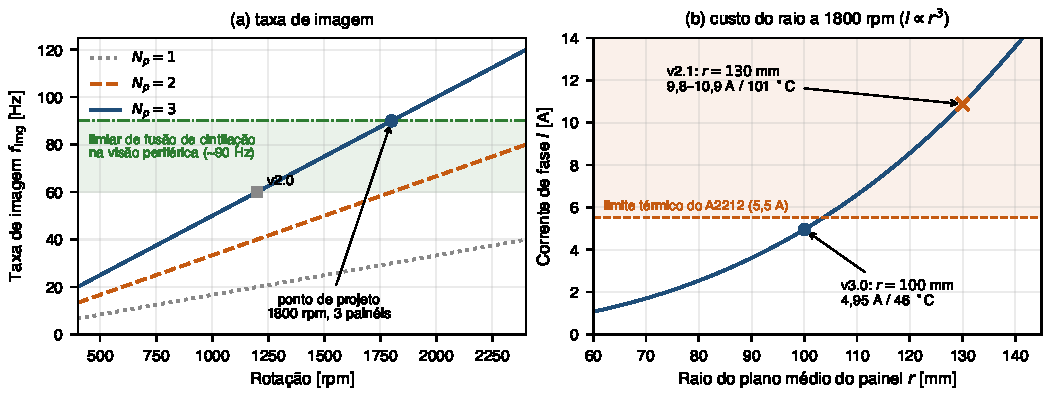
\includegraphics[width=0.98\textwidth]{analise.pdf}
  \caption{Escolha do ponto de operação. (a)~Taxa de imagem em função da
  rotação para 1, 2 e 3 painéis, Eq.~\eqref{eq:fimg}; a faixa em verde marca o
  intervalo de fusão de cintilação. (b)~Corrente de fase em função do raio a
  1800~rpm, Eq.~\eqref{eq:ir3}; a faixa em laranja é a região inviável para o
  A2212 920KV sem ventilação forçada. O alvo de 90~Hz era correto desde a v2.1;
  a variável errada era o raio.}
  \label{fig:analise}
\end{figure*}

\subsection{Esforços no rotor e energia armazenada}

Cada painel de massa $m$ a raio $r$ sofre

\begin{equation}
F_c = m\,\omega^2 r = 0{,}0421 \times 188{,}5^2 \times 0{,}100
\approx 150~\mathrm{N},
\label{eq:fc}
\end{equation}

\noindent carga que é \emph{estática} no referencial do painel: num rotor de eixo
vertical nem a força centrífuga nem o peso mudam de direção em relação à peça,
de modo que não há ciclagem a 30~Hz. O modo de degradação relevante não é
fadiga, e sim fluência do ABS sob carga sustentada a temperatura elevada
\cite{ashby2016}. A energia cinética do rotor,

\begin{equation}
E = \tfrac{1}{2} J \omega^2
  = \tfrac{1}{2} \times 1{,}55\times10^{-3} \times 188{,}5^2
  \approx 27{,}6~\mathrm{J},
\label{eq:energia}
\end{equation}

\noindent e a velocidade tangencial $v=\omega r = 18{,}9$~m/s definem o requisito de
contenção: um painel desprendido carrega cerca de 7,9~J. O desbalanceamento
residual admissível, $U = m\,e$, foi fixado em 8,4~g$\cdot$mm segundo os
procedimentos da ISO~21940-11 \cite{iso21940}, o que se traduz na exigência de
casar as massas dos três painéis dentro de 0,084~g.

\subsection{Dinâmica da estrutura fixa}

A torre é um tubo engastado de rigidez $k \approx 50$~N/mm. Como o centro de
gravidade do conjunto girante fica $a=31$~mm acima do topo do tubo de
comprimento $L$, a rigidez efetiva cai para \cite{rao2018}

\begin{equation}
k_{\mathrm{ef}} = \frac{k}{1 + 3a/L + 3a^2/L^2} \approx 29~\mathrm{N/mm},
\label{eq:keff}
\end{equation}

\begin{equation}
f_n = \frac{1}{2\pi}\sqrt{\frac{k_{\mathrm{ef}}}{m}}
    = \frac{1}{2\pi}\sqrt{\frac{29\,000}{0{,}349}} \approx 46~\mathrm{Hz}.
\label{eq:fn}
\end{equation}

A excitação de desbalanceamento é síncrona, a 30~Hz, o que dá razão de
frequências $f/f_n = 0{,}65$ --- fora da ressonância, mas com margem que
precisa ser confirmada experimentalmente, e não assumida. Daí o ensaio de
impacto previsto na Seção~\ref{sec:metodologia}.

\begin{table}[t]
\centering
\caption{Ponto de operação e grandezas derivadas.}
\label{tab:parametros}
\footnotesize
\setlength{\tabcolsep}{4pt}
\begin{tabular}{@{}lrl@{}}
\toprule
\textbf{Grandeza} & \textbf{Valor} & \textbf{Origem} \\
\midrule
Raio do plano médio, $r$        & 100 mm      & projeto \\
Rotação                          & 1800 rpm    & projeto \\
Velocidade angular, $\omega$     & 188,5 rad/s & $2\pi n$ \\
Painéis, $N_p$                   & 3           & projeto \\
Taxa de imagem                   & 90 Hz       & Eq.~\eqref{eq:fimg} \\
Resolução                        & 29 $\times$ 180 & Eq.~\eqref{eq:passo} \\
Envelope da imagem               & $\varnothing$208 $\times$ 201 mm & CAD \\
Corrente de fase prevista        & 4,95 A      & Eq.~\eqref{eq:ir3} \\
Potência de entrada prevista     & 16,2 W      & fonte \\
Temperatura do motor prevista    & 46 $^\circ$C & Eq.~\eqref{eq:termica} \\
Força centrífuga por painel      & 150 N       & Eq.~\eqref{eq:fc} \\
Energia do rotor                 & 27,6 J      & Eq.~\eqref{eq:energia} \\
Massa do rotor                   & 278,6 g     & CAD \\
Desbalanceamento admissível      & 8,4 g$\cdot$mm & \cite{iso21940} \\
Freq. natural da torre           & 46 Hz       & Eq.~\eqref{eq:fn} \\
\bottomrule
\end{tabular}
\end{table}

% =====================================================================
\section{Objetivos}
% =====================================================================

\subsection{Objetivo geral}

Projetar, construir e validar experimentalmente um display volumétrico por
persistência de visão formado por três painéis de LEDs endereçáveis girando a
1800~rpm, capaz de exibir uma imagem cilíndrica de
$\varnothing$208~$\times$~201~mm com 29~$\times$~180 pixels e taxa de imagem de
90~Hz, operando de forma estável e contida dentro dos limites térmicos,
elétricos e de vibração do conjunto motor--estrutura disponível, com toda cota
e grandeza rastreável até um \emph{datasheet}, uma medição de bancada ou uma
linha de cálculo publicada.

\subsection{Objetivos específicos}

\begin{itemize}
  \item Congelar o ponto de operação da Tabela~\ref{tab:parametros} a partir do
    balanço entre \eqref{eq:fimg}, \eqref{eq:arrasto} e \eqref{eq:termica}.
  \item Entregar o modelo CAD paramétrico com verificação automatizada da
    malha exportada contra os critérios da especificação.
  \item Fabricar e qualificar dimensionalmente o lote de peças, atendendo massa
    $\leq 45$~g por painel, $\Delta m \leq 0{,}084$~g e raio
    $100 \pm 0{,}1$~mm.
  \item Montar e balancear o rotor, com contenção física montada antes de
    qualquer ensaio de rotação.
  \item Aprovar os quatro bloqueadores de rotação da
    Tabela~\ref{tab:bloqueadores}, medidos com instrumentação de bancada.
  \item Integrar a cadeia óptica embarcada e o firmware de varredura,
    sustentando 16,2~mil atualizações de coluna por segundo sem acúmulo de erro
    de fase.
  \item Validar a qualidade visual e documentar operação, ensaios e limitações
    conhecidas.
\end{itemize}

% =====================================================================
\section{Metodologia}
\label{sec:metodologia}
% =====================================================================

A execução é organizada em seis fases separadas por portões de aprovação
(G0 a G5). Um portão é uma condição numérica: enquanto não for atendido, a fase
seguinte não começa. A disciplina existe porque o sistema armazena a energia de
\eqref{eq:energia} e porque os modos de falha relevantes ---
desbalanceamento, sobreaquecimento e perda de sincronismo na partida ---
manifestam-se primeiro como número fora de faixa e só depois como peça
quebrada. Nenhum LED é instalado antes de G3: os ensaios de maior risco físico
são feitos com o mínimo de material embarcado.

\subsection{Projeto paramétrico e verificação do CAD (G0)}

O modelo não é desenhado manualmente. Um programa lê um único arquivo de
parâmetros e constrói base, torre, aranha, painéis, tampa e suporte do ímã
(Figura~\ref{fig:cad}), além de cupons de teste de folga, de modo que uma
mudança de raio se propague por todas as interfaces. A verificação tem duas
camadas: medição da malha exportada contra os critérios da especificação, e
traçado de raios para confirmar que cada furo é vazado de ponta a ponta e que
não restaram membranas dentro de canais --- modo de falha silencioso da geração
booleana, responsável, em revisões anteriores, por furos de parafuso fechados e
por uma lâmina de material de 0,05~mm sob a flange da torre. Uma checagem de
colisões de montagem completa o conjunto. \textbf{G0:} 54 critérios atendidos e
cupons conferidos contra a fita LED real.

\begin{figure}[t]
  \centering
  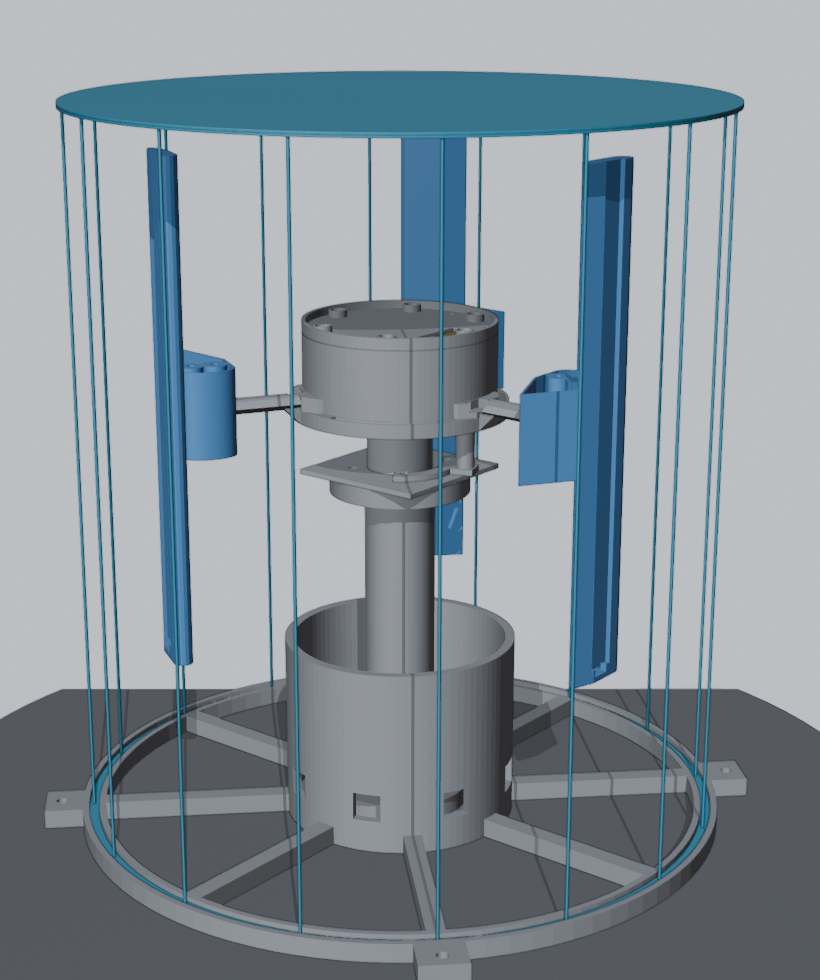
\includegraphics[width=0.70\columnwidth]{cad_montagem.png}
  \caption{Montagem do protótipo no modelo paramétrico (rev.~3.0.3): base
  grampeada, torre, chapa de alumínio, motor, aranha com baia de eletrônica e
  os três painéis no raio de 100~mm. Em transparência, o envelope varrido de
  $\varnothing$208~$\times$~201~mm.}
  \label{fig:cad}
\end{figure}

\subsection{Fabricação e qualificação dimensional (G1)}

Antes do lote definitivo imprimem-se dois cupons --- um da junta painel/longarina
e outro de uma fatia real do canal da fita ---, que custam 25 minutos e evitam
refazer peças de 208~mm por folga errada. Os três painéis são impressos na
mesma mesa, no mesmo lote de filamento e com os mesmos parâmetros, para que
qualquer desvio de processo os afete igualmente. Cada peça é medida com
paquímetro de 0,01~mm e pesada em balança de 0,01~g --- resolução exigida pelo
critério $\Delta m \leq 0{,}084$~g, já que uma balança de 0,1~g mediria
exatamente o tamanho do erro que deveria detectar. Peça fora de tolerância é
reimpressa, não ajustada. \textbf{G1:} massa, $\Delta m$, raio e altura dentro
das tolerâncias.

\subsection{Montagem e balanceamento (G2)}

A ordem é motor na chapa, chapa na flange, aranha no eixo e painéis nas
longarinas. A fixação do rotor exige atenção: o colar de $\varnothing$8~mm do
eixo sobe de 5 a 7~mm acima da campânula, de modo que uma arruela M6 comum
assentaria sobre o colar e a porca não apertaria o cubo. Adota-se arruela
$\varnothing$20~$\times$~$\varnothing$8,5~mm cortada da própria chapa, porca M6
fina e trava química, a 0,6~N$\cdot$m: o atrito necessário para transmitir o
torque exige 22~N, e esse aperto entrega 500~N com tensão de 1,9~MPa no ABS.
Segue o balanceamento estático. Registre-se que casar massas não casa momentos:
0,5~mm de diferença de centro de gravidade em 42~g já vale 21~g$\cdot$mm, duas
vezes e meia o admissível de \eqref{eq:fc}. Quem fecha essa conta é o
bloqueador~C. \textbf{G2:} rotor girando à mão sem rocamento, contenção
montada.

\subsection{Bloqueadores de rotação (G3)}

Executados sem LEDs e sem eletrônica de bordo. Cada um tem critério numérico,
método, limiar de aborto e contingência definidos antes do ensaio
(Tabela~\ref{tab:bloqueadores}). O bloqueador~A sobe em patamares de 600, 1000,
1400 e 1800~rpm, dois minutos em cada, lendo tensão e corrente na fonte; ele
verifica se o arrasto real bate com \eqref{eq:arrasto}, a maior incerteza do
projeto. O~B opera dez minutos contínuos com termopar tipo~K na carcaça e mede,
além da temperatura, o crescimento da deflexão da ponta do painel após uma hora
--- teste direto da fluência prevista em \eqref{eq:fc}. O~C tem duas partes:
ensaio de impacto com massa fictícia de 280~g na altura do plano dos painéis,
para confirmar por FFT a $f_n$ de \eqref{eq:fn}, e medida da vibração residual
em operação. O~D existe porque o rotor tem $J = 1{,}55$~g$\cdot$m$^2$, cerca de
cem vezes a inércia de uma hélice, regime para o qual controladores sem sensor
não são sintonizados.

\begin{table}[t]
\centering
\caption{Critérios de aceite dos bloqueadores de rotação.}
\label{tab:bloqueadores}
\footnotesize
\setlength{\tabcolsep}{4pt}
\begin{tabular}{@{}clr@{}}
\toprule
& \textbf{Grandeza medida} & \textbf{Critério} \\
\midrule
A & Potência de entrada a 1800 rpm & $\leq$ 20 W \\
B & Temperatura do motor, 10 min   & $<$ 55 $^\circ$C \\
B & Crescimento da ponta, 1 h      & $<$ 0,5 mm \\
C & Vibração residual a 30 Hz      & $\leq$ 0,20 g \\
C & Separação $f_n$ / 30 Hz        & confirmada por FFT \\
D & Partidas bem-sucedidas         & 10 de 10 \\
D & Pico de corrente na rampa      & $\leq$ 4,6 A \\
\bottomrule
\end{tabular}
\end{table}

\subsection{Integração óptica e firmware (G4)}

A fita HD107S é alojada no canal dos painéis; a fiação corre pela carenagem e
pela longarina até a baia da aranha, onde ficam o ESP32-C3, o regulador de 5~V,
o deslocador de nível, o capacitor de desacoplamento e a bateria LiFePO$_4$. O
sensor Hall A3144 gira com o rotor e o ímã fica na parte fixa, gerando um pulso
por volta. Duas armadilhas elétricas são tratadas explicitamente: o A3144 não
opera de forma confiável em 3,3~V \cite{allegro_a3144}, e 3,3~V não aciona com
margem as entradas de relógio e dados da fita --- daí o deslocador de nível. O
firmware zera a fase a cada pulso de índice, o que impede acúmulo de erro, e
interpola a posição angular dentro da volta pelo tempo decorrido. Como o
controlador BLHeli\_S não tem malha fechada de rotação, a estabilidade entre
voltas precisa ficar em torno de 0,14\% para manter o desvio abaixo de um quarto
de coluna. Ao fim, o rotor é rebalanceado com a massa real da eletrônica.
\textbf{G4:} imagem de teste estável a 1800~rpm.

\begin{figure*}[!t]
  \centering
  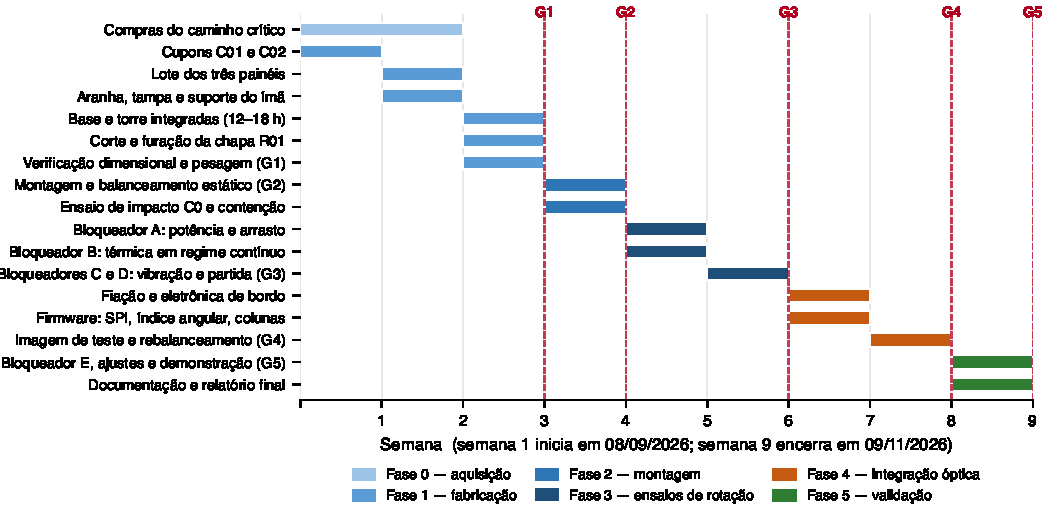
\includegraphics[width=0.90\textwidth]{cronograma.pdf}
  \caption{Cronograma de execução. As linhas tracejadas em vermelho marcam os
  portões de aprovação; nenhuma fase à direita de um portão começa antes que
  seus critérios numéricos sejam atendidos.}
  \label{fig:cronograma}
\end{figure*}

\subsection{Validação visual (G5)}

Ambiente escuro, imagem de teste com grade fina, texto pequeno e bordas
verticais, observada a 1, 2 e 3~m, com olhar parado e em movimento sacádico, e
registrada a 240~quadros por segundo. Critérios: imagem estável, coincidência
das três varreduras e ausência de cintilação periférica. Cada sintoma tem
diagnóstico associado antes da correção --- imagem tripla indica diferença de
raio ou altura entre painéis; deslocamento angular indica folga na junta; borda
serrilhada indica jitter de fase no sensor de índice.


% =====================================================================
\section{Cronograma}
% =====================================================================

O cronograma cobre nove semanas, de 8 de setembro a 9 de novembro de 2026
(Figura~\ref{fig:cronograma}). A Fase~0 --- projeto CAD, memória de cálculo e
verificação --- foi concluída em 5 de setembro de 2026.

O caminho crítico é a impressão da base com a torre integrada: 12 a 18~h em uma
peça única, não paralelizável, e que só pode começar depois de G1, porque uma
correção de raio mudaria a base junto. A folga real está no paralelismo entre
as compras (semana~1) e a impressão (semanas 2 e 3): se a bateria ou o
regulador atrasarem, as fases 1 a 3 seguem sem eles, já que nada em G3 depende
da eletrônica de bordo.


% =====================================================================
\section{Resultados esperados}
% =====================================================================

O projeto será considerado bem-sucedido quando, simultaneamente, a imagem se
formar a 90~Hz sem tremulação perceptível em sacada; a potência de entrada
permanecer em até 20~W com o motor estabilizando abaixo de 55~$^\circ$C; a
vibração a 30~Hz ficar em até 0,20~g sem crescimento; o rotor partir dez vezes
em dez; e toda grandeza do projeto for rastreável até um \emph{datasheet}, uma
medição ou uma linha de cálculo publicada.

Os riscos de maior impacto são o arrasto real acima do estimado em
\eqref{eq:arrasto}, que se manifesta como potência acima de 20~W no
bloqueador~A e cuja mitigação é a carenagem do cubo antes de qualquer redução
de rotação; a fluência do ABS, medida diretamente no bloqueador~B; e a falha de
partida do controlador sem sensor, mitigada por alongamento da rampa e ajuste
das proteções do BLHeli\_S. Caso algum critério não seja atendido, a resposta
prevista não é forçar a operação, e sim reduzir rotação, substituir o
componente crítico ou revisar a geometria --- caminhos já descritos, com ordem
de tentativa, no plano de ensaios do projeto.

% =====================================================================
\begin{thebibliography}{99}
\footnotesize
\setlength{\itemsep}{2.5pt}
\setlength{\parskip}{0pt}

\bibitem{blundell2000}
BLUNDELL, B. G.; SCHWARZ, A. J.
\textit{Volumetric Three-Dimensional Display Systems}.
New York: Wiley, 2000.

\bibitem{favalora2005}
FAVALORA, G. E.
Volumetric 3D displays and application infrastructure.
\textit{Computer}, IEEE, v.~38, n.~8, p.~37--44, 2005.

\bibitem{kelly1961}
KELLY, D. H.
Visual responses to time-dependent stimuli. I. Amplitude sensitivity
measurements. \textit{Journal of the Optical Society of America}, v.~51, n.~4,
p.~422--429, 1961.

\bibitem{tyler1985}
TYLER, C. W.
Analysis of visual modulation sensitivity. II. Peripheral retina and the role
of photoreceptor dimensions. \textit{Journal of the Optical Society of America
A}, v.~2, n.~3, p.~393--398, 1985.

\bibitem{white2011}
WHITE, F. M.
\textit{Fluid Mechanics}. 7. ed. New York: McGraw-Hill, 2011.

\bibitem{hoerner1965}
HOERNER, S. F.
\textit{Fluid-Dynamic Drag}. Bakersfield: edição do autor, 1965.

\bibitem{hendershot2010}
HENDERSHOT, J. R.; MILLER, T. J. E.
\textit{Design of Brushless Permanent-Magnet Machines}.
Oxford: Motor Design Books, 2010.

\bibitem{iso21940}
INTERNATIONAL ORGANIZATION FOR STANDARDIZATION.
\textit{ISO 21940-11: Mechanical vibration --- Rotor balancing --- Part 11:
Procedures and tolerances for rotors with rigid behaviour}. Genebra, 2016.

\bibitem{rao2018}
RAO, S. S.
\textit{Mechanical Vibrations}. 6. ed. Harlow: Pearson, 2018.

\bibitem{ashby2016}
ASHBY, M. F.
\textit{Materials Selection in Mechanical Design}. 5. ed. Oxford:
Butterworth-Heinemann, 2016.

\bibitem{allegro_a3144}
ALLEGRO MICROSYSTEMS.
\textit{A3141/2/3/4 Sensitive Hall-Effect Switches for High-Temperature
Operation --- Datasheet}. Manchester, NH, 2019.

\end{thebibliography}

\end{document}
